\documentclass[tikz, border=1mm]{standalone}

\usetikzlibrary{arrows, shapes.gates.logic.US, calc}
\tikzstyle{branch}=[fill, shape=circle, minimum size=3pt, inner sep=0pt]

\begin{document}
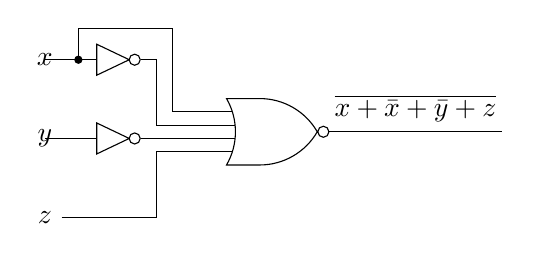
\begin{tikzpicture}
    \node (x) at (0, 2) {$x$};
    \node (y) at (0, 1) {$y$};
    \node (z) at (0, 0) {$z$};

    \node[not gate US, draw] at ($(x) + (0.8, 0)$) (notx) {};
    \node[not gate US, draw] at ($(y) + (0.8, 0)$) (noty) {};

    \draw (x) |- (notx.input);
    \draw (y) |- (noty.input);

    \node[nor gate US, draw, rotate=0, logic gate inputs=nnnn] at ($(noty) + (2, 0.085)$) (xory) {};

    \path ($(notx.input) + (0.2, 0)$) -- coordinate (puntx) (x |- notx);
    \draw (x) |- (puntx) node[branch] {} |- ($(notx.output) + (0.4, 0.4)$) |- (xory.input 1);

    \draw (notx.output) -- ([xshift=0.2cm]notx.output) |- (xory.input 2);
    \draw (noty.output) -- ([xshift=0.2cm]noty.output) |- (xory.input 3);
    \draw (z) -| ($(noty.output) + (0.2, -0.5)$) |- (xory.input 4);

    \draw (xory.output) -- node[above]{$\overline{x + \bar x + \bar y + z}$} ($(xory) + (3, 0)$);
\end{tikzpicture}
\end{document}
